\chapter{Future Enhancements}\label{ch:future-enhancements}

SSL and TLS are protocols for establishing safe and secure connections between networked computers and, today, support
for these protocols is built into most browsers and web servers~\parencite{thomas2000ssl}.
Adding an SSL or TLS certificate to the web app would greatly increase its security, however, it was not possible to
implement such a feature during the deployment of the app.
This was due to the restricted permissions granted to the AWS account used to create this deployment, which
restricted the ability for certain features to be implemented, including the use of certificates.
In future deployments of the web app, it would be greatly beneficial to the security of the app, for both users and the
app itself, to add an SSL or TLS certificate to encrypt the connections to the EC2 instance.
This would be especially important in a future deployment if the user-base would be expected to grow in size.

\begin{figure}[!htbp]
    \centering
    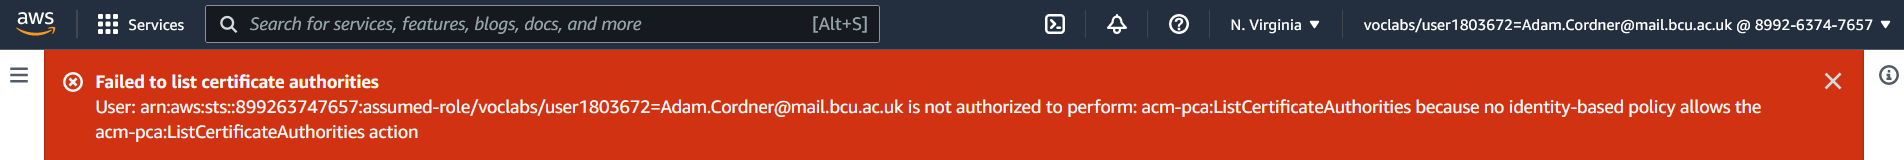
\includegraphics[width=\textwidth]{resources/certificate-denied}
    \caption{Restricted permissions preventing the use of certificates.}
    \label{fig:certificate-denied}
\end{figure}

Another feature which was limited due to restricted permissions was AWS IAM roles.
IAM is an AWS service which provides fine-tuned access control across the entire AWS deployment by creating a policy
which specifies which users have permission to access certain features and resources~\parencite{amazon2022aws2}.
IAM would be very useful if the development team behind \textit{Digital-Ink} was scaled up with future
deployments, and it is especially appealing due to the fact that it is an entirely free service with no additional
costs to use.

\begin{figure}[!htbp]
    \centering
    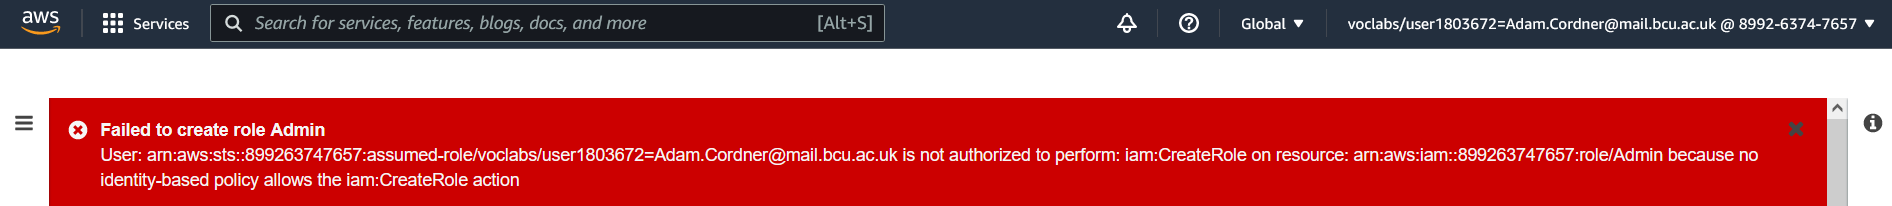
\includegraphics[width=\textwidth]{resources/iam-denied}
    \caption{Restricted permissions preventing the creation of IAM roles.}
    \label{fig:iam-denied}
\end{figure}

\clearpage
Another AWS feature which would be useful in a larger deploy of the web app is AWS Global Accelerator.
Global Accelerator is a service used to optimise user traffic.
Amazon claims that it can improve the performance of user traffic by up to 60\%~\parencite{amazon2022aws4}.
This is useful as it can reduce packet loss, jitter, and latency.
Global Accelerator works by providing two global static IPs, which improves availability, and by adding or removing
endpoints of AWS services, such as ELB, EC2, and Elastic IP, in the backend without making user-facing changes.
Global Accelerator automatically redirects all traffic to the most optimal endpoint.
During the creation of the Load Balancer for this deployment, Global Accelerator was unavailable due to
restricted permissions on the account.
In larger deployments, this service would ideally be used to improve the performance of the web app.

\begin{figure}[!htbp]
    \centering
    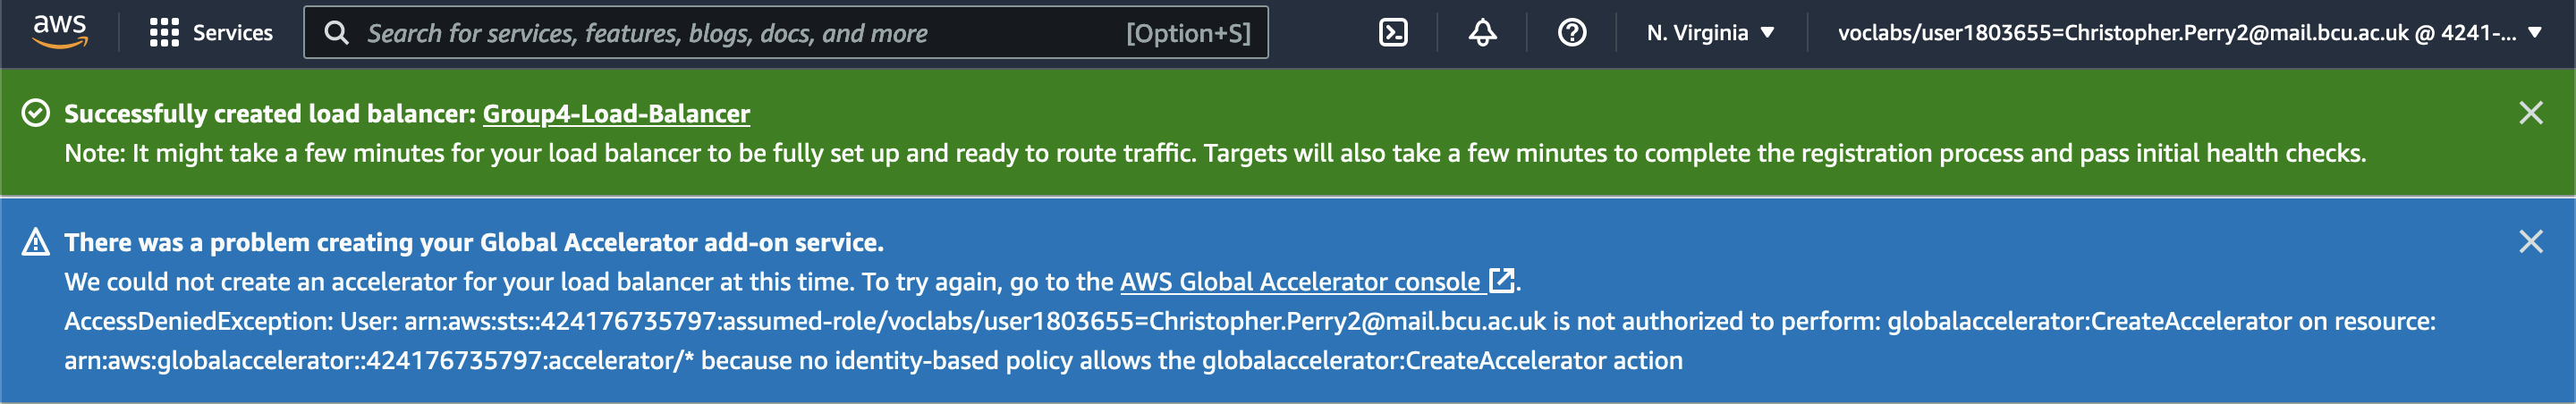
\includegraphics[width=\textwidth]{resources/elb/elb-accelerator}
    \caption{Restricted permissions preventing the creation of Global Accelerator.}
    \label{fig:elb-accelerator}
\end{figure}

If we were to redeploy the app again from scratch, we would consider using AWS Elastic Beanstalk.
EB is a service AWS provides for deploying and scaling web apps automatically.
EB is currently compatible with Java, .NET, PHP, Node.js, Python, Ruby, Go, and Docker~\parencite{amazon2022aws3}.
Considering that \textit{Digital-Ink} uses both PHP and Docker, using EB seems appropriate for future
deployments of the app.
Using EB is simple, simply upload the web app code and EB automatically deploys it, including appropriate
capacity provisioning, load balancing, auto-scaling, and more.
EB can also be used to automatically scale-up and scale-down the web app, which would be useful as the app
grows over time.
In many ways, this automatic handling of the deployment is preferable as it removes the risk of human error
causing the deployment to fail.
This is especially helpful as human error is one of the most significant factors in failed deployments of online
services, and the risk only increases as those services become bigger and harder to manage~\autocite{kraemer2007human}.
Additionally, like IAM, EB has no additional fee to use, as payment is only necessary for the AWS resources
configured by EB, not the use of EB itself.
